\documentclass[titlepage,a4paper,12pt]{article}

\usepackage{texfiles/setup}
\usepackage{config/config}

% Um diese Vorlage zu verwenden, müssen ein paar Einstellungen vorgenommen werden.
% Der Code wird immer aus main.tex compiliert, wenn möglich mit "LuaLaTeX",
% die Gewährleistung der Funktion mit anderen Compilern kann nicht gegeben werden.
%
% Keine Daten im Ordner texfiles verändern, die Eingaben in die Teile wie Titelseite etc.
% erfolgen über die config!
%
% Nach jeder Veränderung an Referenzierungen wie: Label, Überschriften, Zitierungen und 
% Referenzen muss die main.tex ZWEI MAL kompiliert werden um diese zu übernehmen.
% Bei einfacher Kompilation werden die Referenzierungen produziert aber noch nicht übernommen.
% Bei Änderungen am Text o.ä. muss nur einmal kompiliert werden.
%
% Bei erster Benutzung dieser Vorlage zwei Mal mit LuaLaTeX compilieren.
% Anschließend muss einmal wie unter 2. beschrieben die main.tex mit BibTeX compiliert werden, um
% die Referenzierungen zu ermöglichen!
% Dann noch zwei Mal mit LuaLaTeX compilieren um die Vorlagen korrekt in der PDF zu sehen.
%
% Ab hier bei Änderungen LuaLaTeX verwenden, außer es wird die Biblithek verändert.
%
% 1. Bearbeiten der config-Datei unter config/config.sty
%	- Eingabe der Arbeitsdaten wie in der Datei beschrieben
% 2. Anlegen von Bibliotheken (Literatur) in der library-Datei unter config/library.bib
%	- Anlegen von Literatur wie dort vorgegeben oder im Internet nach Vorlagen suchen
%	- Zum Benutzen der angelegten Literatur den Compiler BibTeX in der main.tex laufen lassen
%	- Zitate mit folgendem Code einfügen: \citep[vgl.][S. 508 ff.]{bernstein97}
%		[vgl. ] kann bei direkten Zitaten entfernt werden. bernstein97 ist z.B. das in der library
% 	  	angegebene Referenzwort für das Buch, dieser Alias kann in library.bib frei gewählt werden
% 3. Includieren einzelner Kapitel
%	- Für jedes Kapitel wird eine KAPITELUEBERSCHRIFT.tex im Ordner Chapter erstellt
%	- Jedes Kapitel wird mit \include{chapter/KAPITELUEBERSCHRIFT} im vorgesehenen Bereich
%	    eingefügt
%	- In den Kapiteldateien wird dann der Text geschrieben.
%	- Hierarchie der Überschriften: \section{}, \subsection{}, \subsubsection{}
% 4. Einfügen von Bildern
%	\begin{figure}[ht]
%		\centering
%		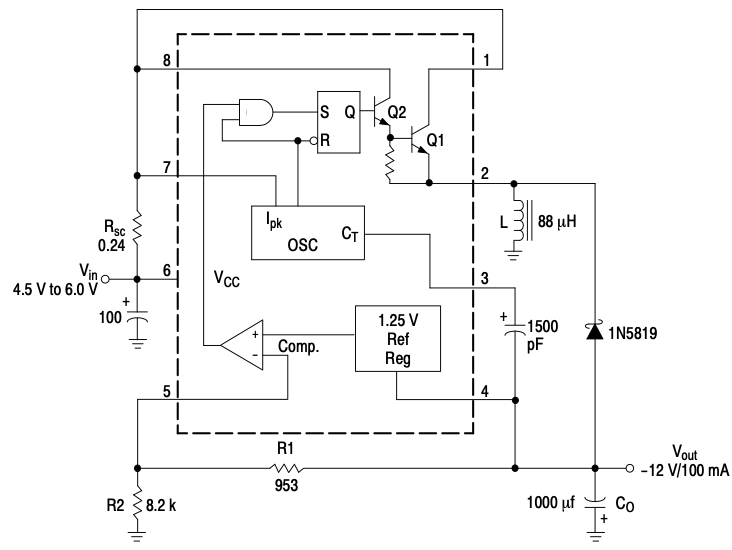
\includegraphics[scale=0.5]{pic/bildname}
%		\caption{Beispielbild}
%		\label{pic:bildname}
%		\quelle \citep[S. 8]{onsemi:MC34063A}
%	\end{figure}
%	- Das Bild wird mit dem vorangegangenen Code eingefügt. Der Dateiname wird unter bildname
% 		angegeben. Mit scale wird manuell nach dem trial-and-error Prinzip die gewünschte Bildgröße 
% 		eingestellt (jedes Mal kompilieren). Die Caption gibt die Bildunterschrift an
% 		Mit label wird ein Alias erstellt, der später mit \ref{pic:bildname} die Zahl des
%		nummerierten Bildes ausgibt. Im Text daher später "wie in Bild \ref{pic:bildname} zu sehen"
%		Der Quelle Befehlt erzeugt eine Quellenunterschrift.
% 5. Hinzufügen von Abkürzungen
%	\acro{cad}[CAD]{Computer Aided Design}
%	- cad ist der Befehl um die Abkürzung aufzurufen, CAD wird im Abkürzungsverzeichnis angezeigt
%		Computer Aided Design wird dann dort ausgeschrieben
%	\ac{cad} zeigt beim ersten Benutzen Computer Aided Design (CAD) und anschließend nur noch CAD. 
% 6. Werden Teile des Dokumentes nicht benötigt (Abkürzungsverzeichnis, Anhang, Tabellenverzeichnis
%		o.ä. dann müssen diese gelöscht werden, an den in dieser Datei kommentierten Punkten dann
%		einfach den jeweiligen Block löschen

\begin{document}

% Include titlepage
% Pre pages before content, use roman numbering
\pagenumbering{Roman}

\begin{titlepage}
	%include fhw logo to right top
	\trimbox{-8.5cm 1.5cm 1cm 1cm}{	
	\begin{tikzpicture}
		
\includegraphics[scale=1]{pic/title/fhw_logo}
	\end{tikzpicture}}	
	\begin{center}
	
		\setmainfont{Calibri}
		\vspace{2.5cm}
    		
    	\textbf{\Huge \conftitle}\\
    	\vspace{0.5cm}
		\textbf{\Huge \conftitletwo}\\
      	
    	\vspace{2.25cm}
		
       	\textbf{\LARGE \confaut}\\
       	\vspace{0.4cm}
       	{\Large \confmatnr}\\ 
       	\vspace{2.25cm}
            
       	{\large\confstudab arbeit im Studiengang \confstud\\
       	\vspace{0.4cm}
       	bei\\
       	\vspace{0.4cm}
       	\confprof\\}       
            
       	\vfill
       
       	\begin{minipage}{0.48\textwidth}
       	\begin{flushleft}
       		{\large\confadrstr\\
       		\confadrort}
       	\end{flushleft}
		\end{minipage}       			       	
		\hfill
       	\begin{minipage}{0.48\textwidth}
       	\begin{flushright}
       		{\large\confstudf\\
       		\confstudftwo}
       	\end{flushright}
		\end{minipage}
		       			       			       	
       	\vspace{1cm}

       	{\large\confdate		\hfill	\confsem. Semester}
   	\end{center}
\end{titlepage}

% Set arial for the rest of the document
\setmainfont{Arial}
	
% Sperrvermerk, entfernen falls kein Sperrvermerk aufgelegt wird	
\setstretch{1.35}
\thispagestyle{empty}
\textbf{\Large Sperrvermerk}

Diese Arbeit enthält vertrauliche Daten und Informationen des Unternehmens, in dem die \confstudab arbeit angefertigt wurde. Sie darf Dritten deshalb nicht zugänglich gemacht werden.

Die für die Prüfung notwendigen Exemplare verbleiben beim Prüfungsamt und beim betreuenden Hochschullehrer.
\newpage

% Inhaltsverzeichnis
\setstretch{1}
\tableofcontents
\sectionmark{Inhaltsverzeichnis}
\newpage

% Abbildungsverzeichnis, Block entfernen falls keine Abbildungen vorhanden
\cleardoublepage\phantomsection\addcontentsline{toc}{section}{\listfigurename}	% TOC Überschrift für Inhaltsverzeichnis
\listoffigures	% Abbildungsverzeichnis einfügen
\sectionmark{Abbildungsverzeichnis}
\newpage

% Tabellenverzeichnis, Block entfernen falls keine Tabellen vorhanden
\cleardoublepage\phantomsection\addcontentsline{toc}{section}{\listtablename}	% TOC Überschrift für Inhaltsverzeichnis
\listoftables	% Tabellenverzeichnis einfügen
\sectionmark{Tabellenverzeichnis}
\newpage

% Formel/Symbol/Indizes-Verzeichnis, Block entfernen falls keine vorhanden
\losheader
\opensymdef	% Erstellen eines Formelzeichens: \newsym[ Beschreibung ]{ befehl }{ Abkürzung }
% Werden nicht sortiert und auch ohne Verwendung eingefügt
% Selbstständige Sortierung: Nach Alphabet, erst lateinisches, dann griechisches
% Befehl darf nicht mit vorhandenem Befehl übereinstimmen, daher außergewöhnlichen Namen wählen oder Prefix verwenden
\newsym[Elektrische Energie]{mEel}{E_{el}}
\newsym[Elektrische Impedanz]{mZ}{Z}
\closesymdef
\listofsymbols
\newpage

% Abkürzungsverzeichnis, Block entfernen falls keine Abkürzungen vorhanden
\acroheader
\begin{acronym} % Erstellen eines Akronyms: \acro{befehlsinhalt}[Abkürzung]{Beschreibung}
% Werden nicht sortiert aber nur bei Verwendung eingefügt		
	\acro{cad}[CAD]{Computer Aided Design}
	\acro{drm}[DRM]{Digital Radio Mondiale}
\end{acronym}
\newpage

% Letzte Einstellungen für den Rest des Textes
\pagenumbering{arabic}
\setstretch{1.35}

% Includes für die einzelnen Kapitel
% Keine Dateiendung verwenden, die Kapitel als .tex file speichern
% \include{chapter/xyz}

\section{Einleitung}
\subsection{Erstes Unterkapitel}
Dies ist ein Zitat:
\lipsum[1-2]
Zwar nicht aus diesem Buch, aber hier eine Zitierung. \citep[vgl. ][S. 5-6]{bernstein97}
\subsection{Zweites Unterkapitel}
Unter Bild \ref{pic:bildname} sieht man eine volle Schönheit.
\begin{figure}[ht]
	\centering
	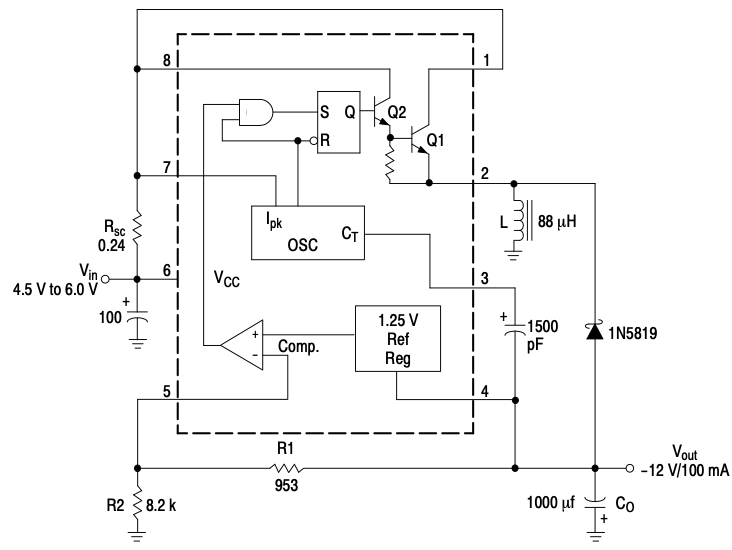
\includegraphics[scale=0.5]{pic/bildname}
	\caption{Beispielbild}
	\label{pic:bildname}
	\quelle \citep[S. 8]{onsemi:MC34063A}
\end{figure}
Ein anderes Bild wird für das Verzeichnis ebenfalls eingefügt.
\begin{figure}[ht]
	\centering
	
\includegraphics[scale=0.5]{pic/title/fhw_logo}
	\caption{Titelbild der FHW}
	\label{pic:titelbild}
\end{figure}

Eine mögliche Abkürzung ist \ac{cad}, sie wird in main.tex definiert. Wenn man dies  ein zweites Mal schreibt, steht nur noch kurz \ac{cad} da. Eine andere Abkürzung wäre \ac{drm}. Möchte man Formelzeichen verwenden, dann deklariert man dieses ebenfalls in main.tex und benutzt dann den dort ausgewählten Befehl. Dieser sollte nur aus Buchstaben bestehen, es darf kein vorhandener Befehl sein. Es ist Empfehlenswert im Befehl m vorweg zu verwenden, um eine mögliche Befehlsüberschneidung auszuschließen. Das Symbol sieht dann so aus: \mEel.

\subsection{Drittes Unterkapitel}
\section{Neuer Abschnitt}
\lipsum[1-3]

Zum Abschluss sollen noch zwei Tabellen dargestellt werden:
\begin{table}[H]
\centering
\begin{tabular}{c c}
Zelle 11 & Zelle 12\\
Zelle 21 & Zelle 22\\
\end{tabular}
\caption{Eine Tabelle}
\label{tab:einetabelle}
\quelle Unbekannt
\end{table}

Die Zweite:
\begin{table}[H]
\centering
\begin{tabular}{l c r}
Zelle 11 & Zelle 12 & Zelle 13\\
Zelle 21 & Zelle 22 & Zelle 23\\
Zelle 31 & Zelle 32 & Zelle 33\\
\end{tabular}
\caption{Eine weitere Tabelle}
\label{tab:eineweiteretabelle}
\end{table}




% Abspannseiten: Literaturverzeichnis, Anhang und Eigenständigkeitserklärung

\newpage
% Set page numbering to roman
\pagenumbering{roman}

% Literaturverzeichnis
\bibliographystyle{agsm}
\bibliography{config/library}
\newpage

% Anhang, entfernen falls kein Anhang vorhanden
\include{chapter/anhang}
\newpage

% Abschlusserklärung
\setcounter{secnumdepth}{0}
\section{Erklärung}

Hiermit erkläre ich, dass ich die von mir eingereichte \confstudab arbeit "\conftitle\  \conftitletwo "\ selbständig und nur unter Verwendung der angegebenen Quellen und Hilfsmittel angefertigt habe.

\vspace{1.5cm}

\confuort, den \confudate

\vspace{3.5cm}




\confaut

\end{document}
